\documentclass[12pt]{article}
\usepackage[shortlabels]{enumitem}
\usepackage{float}
\usepackage{xcolor}
\usepackage[a4paper, top=1.5cm, bottom=1.5cm, left=2cm, right=2cm]{geometry}
\usepackage{parskip}
\usepackage{setspace}
\usepackage{lmodern}
\usepackage[T1]{fontenc}
\usepackage[brazil]{babel}
\usepackage{hyperref}
\usepackage{graphicx}
\usepackage{amsmath}
\usepackage{amssymb}
\usepackage{amsfonts}
\usepackage{dsfont}
\usepackage{float}
\title{Lista 2 - Estatística para Administração - 2025.2}
\begin{document}
\date{}
\maketitle

1) Consiste em realizar afirmações acerca da população a partir da amostra. 
Não podemos realizar inferência baseada em uma amostra gerada por um método não probabilístico.
O uso de métodos não probabilísticos invalida diversos pressupostos que são base para a realização de inferência. Esse ponto será discutido com maior profundidade quando 
estudarmos o processo de inferência estatística. 
\vspace{5px}

2) Determine o valor numérico das seguintes expressões:

\begin{enumerate}[a)]
    \item $\sum\limits_{i = 1}^3 i = 6$
    \item $\sum\limits_{i = 1}^5 i^2 = 55$
    \item $\sum\limits_{i = 1}^4 \dfrac{1}{i} = \frac{25}{12}$
    \item $\sum\limits_{i = 1}^4 (-1)^{i} = 0$
    \item $\sum\limits_{i = 1}^3 4x = 12x$
    \item $\sum\limits_{i = 1}^n (-1)^{i}$ onde $n$ é par $=0$
    \item $\sum\limits_{i = 1}^n (-1)^{i}$ onde $n$ é ímpar $=-1$
    \item $\prod\limits_{i=1}^5 (i-1)^2 = 0$
    \item $\prod\limits_{i=1}^3 2^i = 64$
    \item $\prod\limits_{i=1}^n -1$ onde $n$ é par $=1$
    \item $\sum\limits_{x \in \{ 1, 2,5,6,20,10\}} x = 44$
    \item $\sum\limits_{s \in \{ 2,4,6,8,10\}}  \dfrac{e^s}{\sum\limits_{m \in \{ 2,4,6,8,10\}} e^m}  = 1$
    \item $\sum\limits_{i=1}^5\sum\limits_{j=1}^3 2^j = 70$
    \item $\sum\limits_{i=1}^5\sum\limits_{j=0}^i 3^{(j-1)} = \frac{542}{3}$
\end{enumerate}
\vspace{5px}

3) Considere o seguinte conjunto de dados referente a uma pesquisa realizada com estudantes da Praia Vermelha acerca da participação em Empresa Júnior:

\begin{table}[H]
\centering
\begin{tabular}{llll}
\hline
Nome     & Idade & Curso          & E.Junior \\ \hline
Matheus  & 22    & Economia       & 1        \\
Pawel    & 31    & Administração  & 0        \\
Jean     & 29    & Administração  & 1        \\
Janaina  & 18    & Contabilidade  & 1        \\
Leandro  & 19    & Psicologia     & 0        \\
Karolina & 62    & Psicologia     & 0        \\
Katarina & 41    & Administração  & 1        \\
Gilberto & 22    & Economia       & 1        \\
Maya     & 27    & Serviço Social & 1        \\ \hline
\end{tabular}
\end{table}

A coluna E.Junior indica se o estudante participa ou não de Empresa Júnior. 1 - Sim e 0 Não.

\begin{enumerate}[a)]
    \item $\bar{x}=30,11$. Fornecer apenas a média não é suficiente para entender a variável, pois a média pode ser distorcida pela presença de pontos aberrantes, além de não descrever a variabilidade dos valores assumidos pela variável. 
    
    \item \begin{table}[H]
    \centering
    \begin{tabular}{llll}
    \hline
    Curso          & $n_i$ & $f_i$  & $f_{ac}$ \\ \hline
    Economia       & 2     & 0,2222 & 0,2222   \\
    Administração  & 3     & 0,3333 & 0,5555   \\
    Psicologia     & 2     & 0,2222 & 0,7777   \\
    Contabilidade  & 1     & 0,1111 & 0,8888   \\
    Serviço Social & 1     & 0,1111 & 1        \\
    Total          & 9     & 1      &          \\ \hline
    \end{tabular}
    \end{table}
    
    A variável Curso é qualitativa nominal. A variável Nome também é qualitativa nominal.
    
    \item $Q_2 = 27$. A mediana é menor que a média, indicando que a maior parte dos dados (pelo menos 50\%) está localizada antes da média. Ademais, 
    o fato da mediana estar distante três unidades à esquerda pode indicar a presença de valores aberrantes que podem estar fazendo com que o valor da média seja jogado para cima.
    
    \item $\hat{p} = 6/9 \approx 0,67$. $\hat{p}$ representa a proporção amostral de alunos que participam de Empresa Júnior. 
    
    \item $\varepsilon = 0$. Essa métrica não tem nenhum sentido prático. Conforme vimos em sala, independentemente do conjunto, essa métrica sempre resulta em zero, logo não tem nenhuma utilidade prática. 
\end{enumerate}

\vspace{5px}

4) Considere o gráfico a seguir referente à nacionalidade dos estudantes que prestaram o ENEM no ano de 2022. 

\begin{figure}[H]
    \centering
    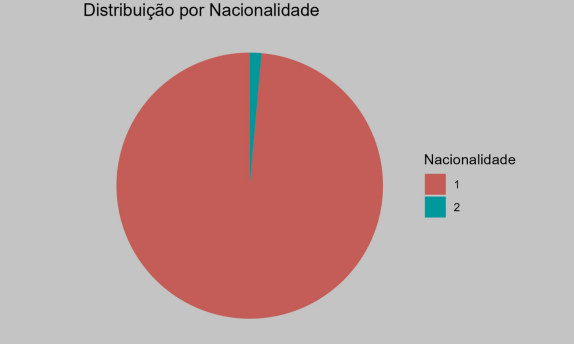
\includegraphics[width=0.4\linewidth]{figures/pizza_1_exercicio.png}
\end{figure}

Podemos notar alguns problemas no gráfico acima. Dentre eles, vale destacar o uso inadequado do gráfico de pizza. Em aula, vimos que, apesar de não ser proibido, não recomenda-se 
o uso de gráficos de pizza, mas, caso seja estritamente necessário usá-lo, devemos ao menos colocar uma legenda indicando as porcentagens, coisa que não ocorre no gráfico acima. 
Além disso, um erro grave cometido nesse gráfico é usar números para representar a nacionalidade, mas não informar o que cada número significa. Como se trata do ENEM, é 
razoável assumir que o número 1 provavelmente representa a nacionalidade brasileira, já a 2 não fica claro, pode ser que 2 sejam outras nacionalidades ou então uma nacionalidade
específica, não dá para saber. Ainda nesse sentido, um leitor de outro país, um imigrante ou alguém que não conhece o ENEM, poderia acabar não fazendo a associação 
de que o número 1 significa brasileira. A resposta para qual visualização usar ao invés da apresentada é bastante ampla. Pessoalmente, se fosse um artigo escreveria 
as porcentagens por extenso em um pequeno parágrafo, deixando bem claro as nacionalidades envolvidas. Se fosse uma apresentação em uma empresa, eu usaria os números como 
big numbers, ou seja, números destacados e em fontes estilizadas. Para quem se interessar, uma discussão maior sobre como escolher gráficos pode ser encontrada no livro 
Storytelling com Dados: um Guia Sobre Visualização de Dados Para Profissionais de Negócios da autora Cole Nussbaumer Knaflic.

\vspace{5px}

5) Considere o gráfico a seguir referente ao acompanhamento de indivíduos com insuficiência cardíaca. 

\begin{figure}[H]
    \centering
    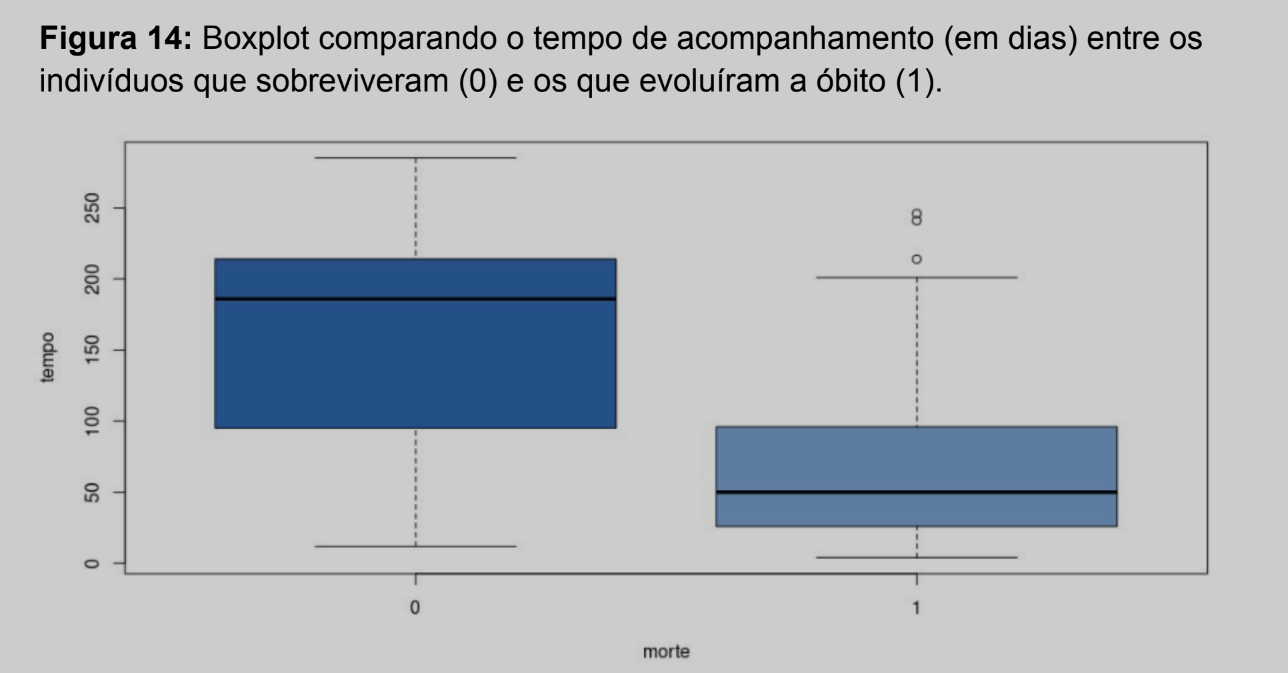
\includegraphics[width=0.6\linewidth]{figures/boxplot_2.png}
\end{figure}

A imagem acima é um gráfico de boxplot evidenciando a distribuição da variável tempo de acompanhamento em relação à variável morte, onde 0 indica sobrevivência e 1 morte. 
Podemos notar que a mediana do tempo de acompanhamento para os indivíduos que sobreviveram é maior que a dos que morreram, ou seja, pelo menos 50\% dos indivíduos que sobreviveram tiveram um tempo
de acompanhamento inferior a 200, enquanto para os mortos o valor foi igual a 50. Ainda nesse sentido, nota-se que o primeiro quartil para os indivíduos sobreviventes é superior ao terceiro quartil
dos que morreram, indicando uma informação bastante crítica, de que 75\% dos indivíduos que morreram tiveram tempos de acompanhamento semelhantes à aproximadamente 25\% dos que sobreviveram. Ademais, focando especificamente no boxplot dos indivíduos que sobreviveram, nota-se 
um comportamento assimétrico. A distância entre o segundo quartil e o terceiro é menor que a entre o primeiro e o segundo, indicando que o tempo de acompanhamento
varia mais abaixo do segundo quartil do que acima. Outro ponto que merece destaque é a presença de outliers no boxplot dos indivíduos que faleceram, enquanto, por 
outro lado, não há a presença de outliers no boxplot dos indivíduos que sobreviveram.

\vspace{5px}

6) 

$$(a+b)^5 = a^5 + 5a^4b + 10a^3b^2 + 10a^2b^3 + 5ab^4 + b^5$$
\vspace{5px}

7) Questão prática. Se tiverem dúvidas basta mandar um e-mail. 

\end{document}